%\VignetteIndexEntry{Exercise 04 from Seminar III: R/Bioconductor}
%\VignetteDepends{}
%\VignetteKeywords{R, Bioconductor}
%\VignettePackage{SIII: R/Bioc}
\documentclass[letterpaper,12pt]{article}

%%%%%%%%%%%%%%%%%%%%%%%% Standard Packages %%%%%%%%%%%%%%%%%%%%%%%%%%%%%%%%%%%%%%%%%%
%\usepackage{epsfig}
%\usepackage{graphicx}
%\usepackage{graphics}
%\usepackage{amssymb}
%\usepackage{amsmath}
%\usepackage{mathrsfs}
%\usepackage{caption}
%\usepackage{comment}
\usepackage{fancyvrb}
\usepackage{fancyhdr}

\usepackage[a4paper]{geometry}
\usepackage{hyperref,graphicx}

%\usepackage[spanish]{babel}
%\selectlanguage{spanish}
%\usepackage[utf8]{inputenc}

%%%%%%%%%%%%%%%%%%%%%% some personal commands %%%%%%%%%%%%%%%%%%%%%%%%%%%%%%%%%%%%%%%%%%%%
\newcommand{\pl}[1]{\texttt{#1}}
\newcommand{\myurlshort}[2]{\href{http://#1}{{\textsf{#2}}}}

%%%%%%%%%%%%%%%%%%%%%% headers and footers %%%%%%%%%%%%%%%%%%%%%%%%%%%%%%%%%%%%%%%%%%%%
\pagestyle{fancy} 
\renewcommand{\footrulewidth}{\headrulewidth}

%%%%%%%%%%%%%%%%%%%%%%%%% bibliography  %%%%%%%%%%%%%%%%%%%%%%%%%%%%%%%%%%%%%%%%%%%%%%%
\bibliographystyle{plainnat}

%%%%%%%%%%%%%%%%%%%%%%%%% sweave options  %%%%%%%%%%%%%%%%%%%%%%%%%%%%%%%%%%%%%%%%%%%%%%%




%%%%%%%%%%%%%%%%%%%%%%% opening %%%%%%%%%%%%%%%%%%%%%%%%%%%%%%%%%%%%
\title{\textbf{Seminar III: \texttt{R}/\texttt{Bioconductor}\\ \small August-December 2009}}
\author{Leonardo Collado Torres\\[1em]Bachelor in Genomic Sciences (LCG),\\ UNAM, Cuernavaca, Mexico\\[1em]\texttt{lcollado@lcg.unam.mx}\\[1em]\url{http://www.lcg.unam.mx/~lcollado/}}

\usepackage{Sweave}
\begin{document}
\maketitle

\medskip
\noindent{\small\textbf{Assistants:} Alejandro Reyes \pl{areyes@lcg.unam.mx}, Jos\'e Reyes \pl{jreyes@lcg.unam.mx} and V\'ictor Moreno \pl{jmoreno@lcg.unam.mx}}

\medskip
\noindent{\small\textbf{Note:} Questions through the \myurlshort{foros.nnb.unam.mx/viewforum.php?f=111}{forum} please. Those who are not from the sixth LCG generation send us an email so we can register you on the forum.}

\medskip
\noindent{\small\textbf{Note:} I changed the original homework due to some unexpected errors with Uniprot using biomaRt and because the ENSEMBL tutorial was outdated.}


\medskip
\begin{abstract}
With the following exercises you'll tune your skills with packages such as biomaRt that enable you to download public data sets.
\end{abstract}

\section{biomaRt}
  \begin{enumerate}
  \item On the class we made the following xyplot. Reproduce it for Bacillus anthracis Sterne and Escherichia coli O17:K52:H18 UMN026
\begin{Schunk}
\begin{Sinput}
> library(biomaRt)
> library(lattice)
> bsub <- useMart("bacterial_mart_54", dataset = "bac_6_gene")
> res <- getBM(attributes = c("start_position", "end_position", 
+     "strand", "status"), filters = c("start", "end"), values = list("1", 
+     "100000"), mart = bsub)
> print(xyplot(end_position ~ start_position | status, group = strand, 
+     data = res, auto.key = T, main = "B. subtilus"))
\end{Sinput}
\end{Schunk}
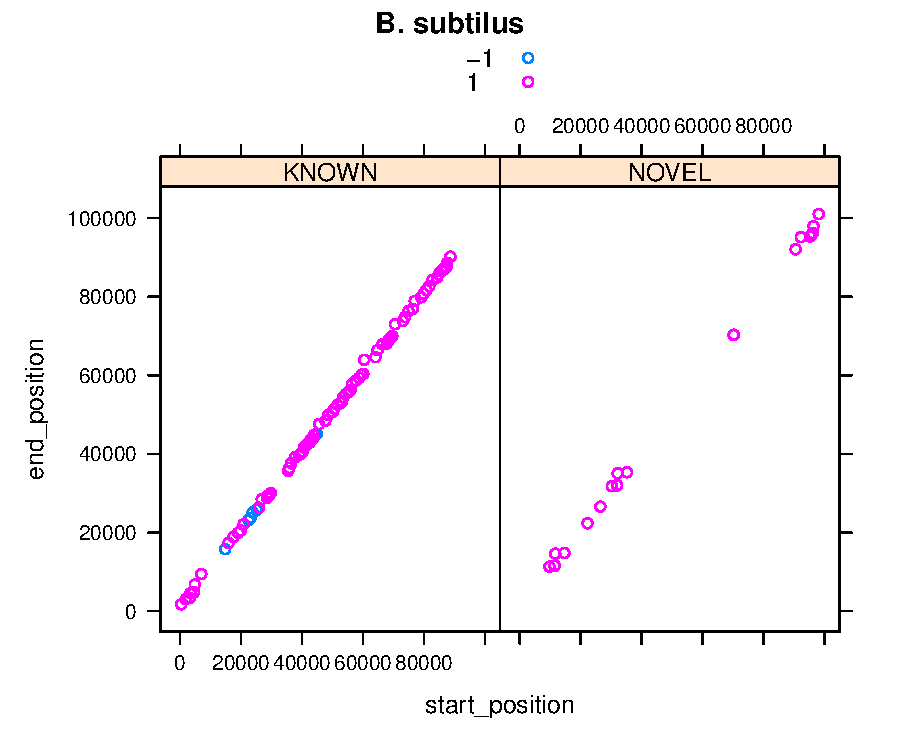
\includegraphics{plots/fig-001}
\begin{Schunk}
\begin{Sinput}
> coli <- useMart("bacterial_mart_54", dataset = "esc_32471_gene")
> res2 <- getBM(attributes = c("start_position", "end_position", 
+     "strand", "status"), filters = c("start", "end"), values = list("1", 
+     "100000"), mart = coli)
> print(xyplot(end_position ~ start_position | status, group = strand, 
+     data = res2, auto.key = T, main = "E. coli 017:K52:H18 UMN026"))
\end{Sinput}
\end{Schunk}
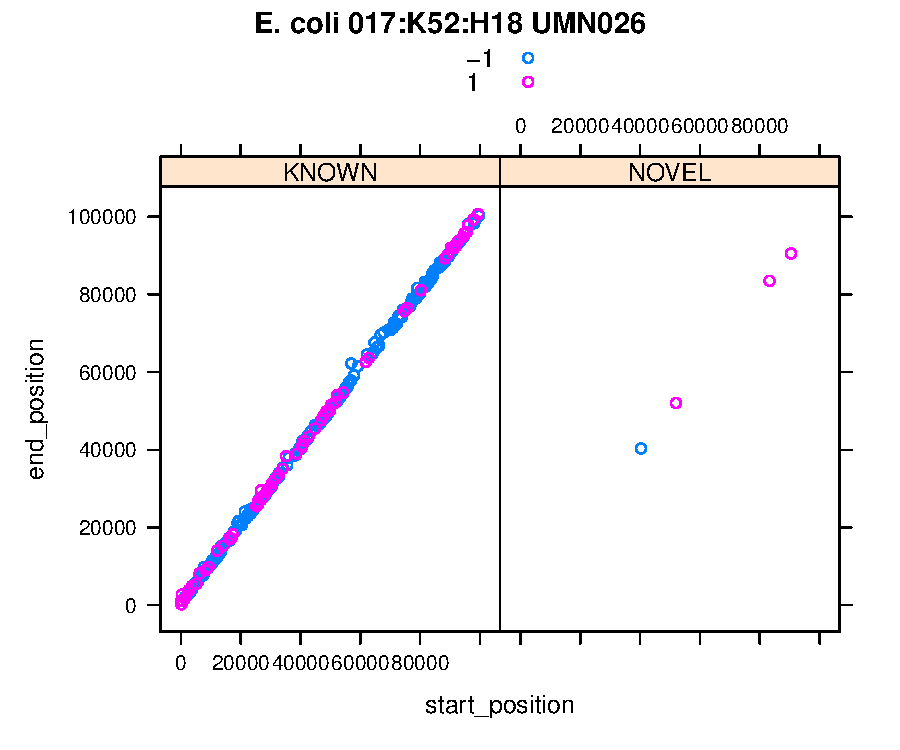
\includegraphics{plots/fig-002}
\begin{Schunk}
\begin{Sinput}
> anthrax <- useMart("bacterial_mart_54", dataset = "bac_20000_gene")
> res3 <- getBM(attributes = c("start_position", "end_position", 
+     "strand", "status"), filters = c("start", "end"), values = list("1", 
+     "100000"), mart = anthrax)
> print(xyplot(end_position ~ start_position | status, group = strand, 
+     data = res3, auto.key = T, main = "B. anthracis"))
\end{Sinput}
\end{Schunk}
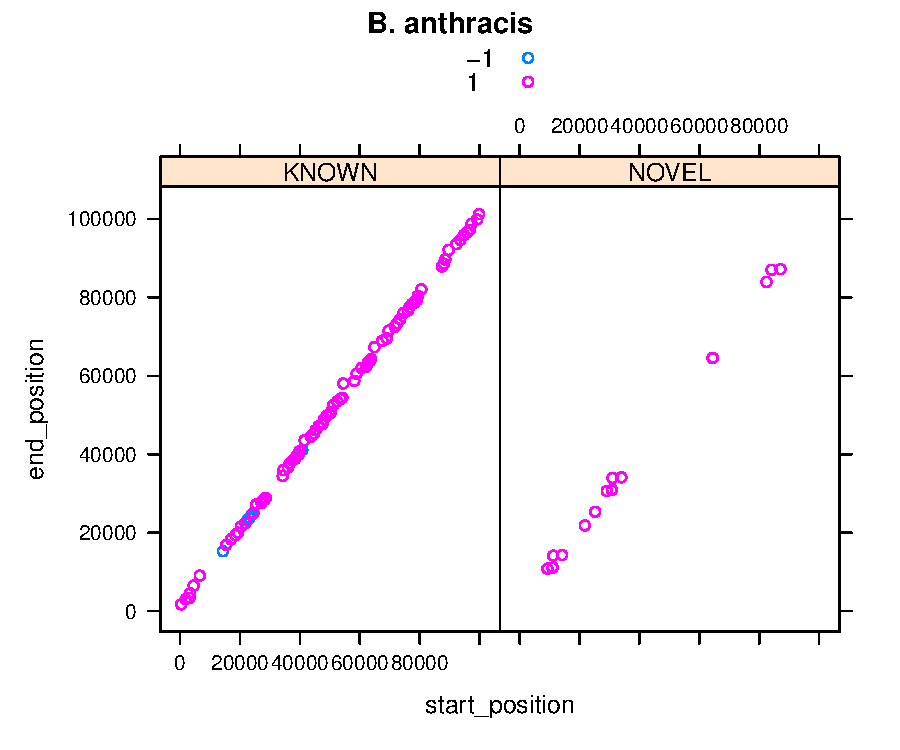
\includegraphics{plots/fig-003}
  \item Compare the three plots and the resulting data sets. Write your own conclusions
\begin{Schunk}
\begin{Sinput}
> dim(res)
\end{Sinput}
\begin{Soutput}
[1] 110   4
\end{Soutput}
\begin{Sinput}
> dim(res2)
\end{Sinput}
\begin{Soutput}
[1] 262   4
\end{Soutput}
\begin{Sinput}
> dim(res3)
\end{Sinput}
\begin{Soutput}
[1] 101   4
\end{Soutput}
\end{Schunk}
B. subtilus and B. anthracis have a nearly the same number of genes on the first 100000bp with B. subtilus having 9 more and a total of 110. Both have a very strong bias for the + strand with the great majority being of known type. E. coli 017:K52:H18 UMN026 has only 4 novel genes but overall has 262 genes on the same subset, which more than doubles any of the other two bacteria. On the xyplot this fact is reflected by a higher density of points, and there seems to be no bias on the strand. Some parts have genes on both strands, though we can clearly notice some segments where nearly all the genes are on one strand; specially on the - strand. 
  \end{enumerate}


\end{document}
